\documentclass[11pt,a4paper]{article}
\usepackage[utf8]{inputenc}
\usepackage{amsmath}
\usepackage{amsthm}
\usepackage{xcolor}
\usepackage{amsfonts}
\usepackage{amssymb}
\usepackage{makeidx}
\usepackage{graphicx}
\author{Todor Antic}
\title{Combinatorics}
\newtheorem{thm}{Theorem}
\newtheorem{ex}{Example}
\newtheorem{sol}{Solution}
\newtheorem{defn}{Definition}
\newcommand{\addbinomial}[3][2]{(#2 + #3)^#1}
\usepackage{caption}
\captionsetup{justification   = raggedright,
	singlelinecheck = false}
\begin{document}
	\maketitle
	\tableofcontents
	\newpage
	
	\section{What is combinatorics?}
	\begin{defn}
		\textcolor{red}{Combinatorics is a branch of mathematics that studies (usually finite) collections of objects that satisfy specified criteria.\cite{dic}}
	\end{defn}
	In simpler terms combinatorics is the mathematics of counting and ar-
	ranging. Of course, most people know how to count, but combinatorics ap-
	plies mathematical operations to count quantities that are much too large
	to be counted the conventional way.
	Combinatorics is especially useful in computer science. Combinatorics
	methods can be used to develop estimates about how many operations a
	computer algorithm will require. Combinatorics is also important for the
	study of discrete probability. 
	
	\subsection{Basic objects of study in combinatorics}
	When studying combinatorics, the most basic objects of study are:
	\begin{enumerate}
		\item Factorials
		\item Combinations
			\begin{enumerate}
				\item Without repetition
				\item With repetition 
			\end{enumerate}
		\item Permutations
			\begin{enumerate}
				\item Without repetition
				\item With repetition 
			\end{enumerate}
	\end{enumerate}

	\subsection{Factorials}
	Combinatorics can help us count the number of orders in which something can happen. Consider the following example:
	\begin{ex}
		In a classroom there are 3 UP Famnit Students and 3 computers standing in a row. In how many different orders can the students use the computers?
	\end{ex}
	\begin{sol}
		Let us list all the possibilities for Student 1 using computer 1 (tables \ref{tab: First} and \ref{tab: Second})\\
		
		\begin{table}
			
			\begin{tabular}{cc|c|c|c|}
				& \multicolumn{1}{c}{}  \\
				& \multicolumn{1}{c}{} & \multicolumn{1}{c}{$St. 1$}  & \multicolumn{1}{c}{$St. 2$}  & \multicolumn{1}{c}{$St. 3$} \\\cline{3-5}
				& $C1$ & USE & NO & NO \\ \cline{3-5}
				& $C2$ & NO & USE & NO \\\cline{3-5}
				& $C3$ & NO & NO & USE \\\cline{3-5}
			\end{tabular}
			\label{tab: First}
			\caption{First possibility}
		\end{table}
	
	\begin{table}
		
		\begin{tabular}{cc|c|c|c|}
			& \multicolumn{1}{c}{}  \\
			& \multicolumn{1}{c}{} & \multicolumn{1}{c}{$St. 1$}  & \multicolumn{1}{c}{$St. 2$}  & \multicolumn{1}{c}{$St. 3$} \\\cline{3-5}
			& $C1$ & USE & NO & NO \\ \cline{3-5}
			& $C2$ & NO & NO & USE \\\cline{3-5}
			& $C3$ & NO & USE & NO \\\cline{3-5}
		\end{tabular}
		\label{tab: Second}
		\caption{Second possibility}
	\end{table}
	
		
		We notice that there is 2 possibilities when Student 1 is using Computer 1, if we write down all the possibilities we'll see that same goes for him using computers 2 and 3. Therefore there is 6 total possibilities. That is because when we're assigning computers to students we have 3 possible students for computer 1, 2 for computer 2 and  1 for computer 3. Than we have $3 \cdot 2 \cdot 1 = 6$ possibilities. 
		 
	\end{sol}
This number is called 3 factorial and is noted as $3!$. Factorials are frequently used when studying combinatorics. 

	\subsection{Combinations}
	Combinations are mathematical objects created by collecting items from a
	group or a set into different groups or sets. It is important to note that
	when taking combinations we do not consider the order of objects
	
	\subsubsection{Calculating the number of combinations}
	\begin{equation} \label{cwr}
	C_n^k=\frac{n1}{(n-k)! \cdot k!)}={n\choose k}, \qquad 0\le k\le n
	\end{equation}

	Equation \eqref{cwr} is used to calculate the number of combinations without repe-
	tition in set with $n$ elements with $k$ elements in each combination. In other words, this way we calculate the number of ways to take $k$ elements from a set with cardinality $n$, without taking any element more than once. ${n \choose k}$ is a common notation.
	
	\begin{equation} \label{cr}
	\overline C_n^k={n+k-1\choose k}
	\end{equation}
	Equation \eqref{cr} is used to calculate the number of combinations with repetition.
	
	\subsection{Permutations}
	Permutations are mathematical objects created by arranging items from
	a group of set into another group of set, taking the order of objects into
	consideration.
	
	\subsubsection{Calculating the number of permutations}
	\begin{equation}\label{pwr}
	P_n=n\cdot\left(n-1\right)\cdots 3\cdot 2\cdot 1=n!
	\end{equation}
	
	Equation \eqref{pwr} is used to calculate the number of permutations of set with n
	elements without repetition. As shown in the figure \ref{fig : Perm}. \\ 
	
	\begin{equation}\label{pr}
	\overline P_n^{n_1,n_2,\ldots ,n_m}=\frac{n!}{n_1!\cdot n_2!\cdots n_m!},\qquad n_1+n_2+\cdots +n_m=n,\qquad 0\le m\le n
	\end{equation}
	Equation (4) is used to calculate the number of permutations with repeti-
	tion on set with $n$ elements of which there is $m$ different ones. If set $A$ with
	cardinality $n$ has $m$ different elements $a_1 , a_2 , \ldots , a_m$ , we calculate of possible
	ways to arrange $a_1 , a_2 , \ldots , a_m $ with $n_i$ being the number of occurrences of
	$a_i$ in each of the permutations.
	
	\begin{figure}[h]
		
		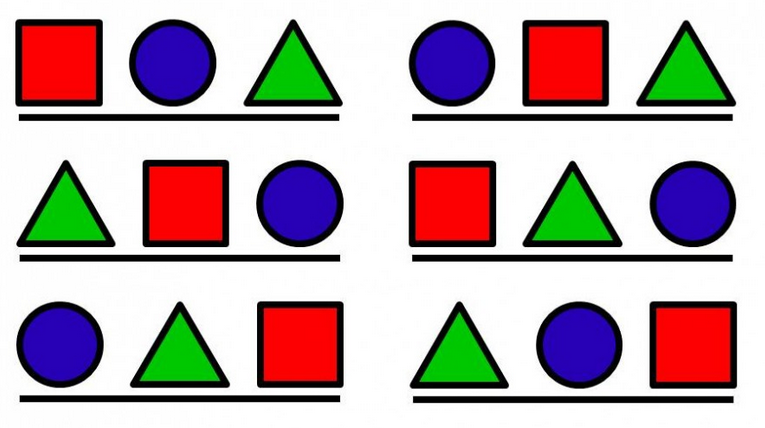
\includegraphics[scale=0.2]{permutations.png}
		\caption{Permutations without repetition}
		\label{fig : Perm}
		
		
	\end{figure}

\section{Binomal theorem}

\begin{thm}
	\begin{multline}
	(a + b)^n = \sum_{k=0}^{n}{n \choose k}a^{n-k}b^k  \\= {n \choose 0}a^n + {n \choose 1}a^{n-1}b + \, \cdots \, + {n \choose n-1}ab^{n-1} + {n \choose n}b
	\end{multline}
\end{thm}
\begin{proof}
	One can establish a bijection between the products of a binomial
	raised to $n$ and the combinations of $n$ objects. Each product which results
	in $a^{n-k}b^k$ corresponds to a combination of $k$ objects out of $n$ objects. Thus, each  $a^{n-k} b^k$ term in the polynomial expansion is derived from the sum of ${n \choose k}$ products.
\end{proof}

\begin{ex}
	Expansions of $(a+b)^n$ for $n \in \{1,2,3,4\}; \, n \in \mathbb{N}$
	\begin{eqnarray}
	&\addbinomial[0]{a}{b}& = \, 1 \nonumber \\
	&\addbinomial[1]{a}{b}& = \, a + b \nonumber\\
	&\addbinomial[2]{a}{b}& = \, a^2 + 2ab + b^2 \nonumber \\
	&\addbinomial[3]{a}{b}& = \, a^3 + 3a^2b + 3ab^2 + b^3 \nonumber \\
	&\addbinomial[4]{a}{b}& = \, a^4 + 4a^3b + 6a^2b^2 + 4ab^3 + b^4 \nonumber  
	\end{eqnarray}
\end{ex}

\section{Pascal triangle}
Take into consideration coefficients from Example 1, if we write them down
we’ll get something like this: 
\\ \\
\begin{tabular}{rccccccccc}
	$n=0$:&    &    &    &    &  1\\\noalign{\smallskip\smallskip}
	$n=1$:&    &    &    &  1 &    &  1\\\noalign{\smallskip\smallskip}
	$n=2$:&    &    &  1 &    &  2 &    &  1\\\noalign{\smallskip\smallskip}
	$n=3$:&    &  1 &    &  3 &    &  3 &    &  1\\\noalign{\smallskip\smallskip}
	$n=4$:&  1 &    &  4 &    &  6 &    &  4 &    &  1\\\noalign{\smallskip\smallskip}
\end{tabular}
\\
Also notice that: \\
First row is: \, \, \qquad $C_0^1$ \\
Second row: \, \, $C_0^1$ \qquad $C_1^1$ \\
Third row: $C_0^2$ \qquad $C_1^2$ \qquad $C_2^2$ \\
and so on.
\\ 
\\
Now we also know that the $k^th$ number in the $n^th$ row is also given by
$C_k^n$ (but we always have to start counting at $0$, so the first row or column is
actually the $\text{zero}^th$ row). If we apply what we know about creating Pascal’s
triangle to our combinations, we get:
$$ {n \choose k} + {n \choose k+1} = {n+1 \choose k+1}$$
This is known as Pascals identity. 

\section{Proving the Pascals identity}
Pascals identity can be proven algebraically, but as that is quite complicated
we’ll show a much simpler and cleaner way of proving it: \\

\begin{proof}
	Let $S$ be a set with $n + 1$ elements, and consider some fixed $x \in S$.
	There are ${n+1 \choose k}$ $k$-subsets of $S$, count them according to whether or not they
	contain $x$: there are ${n \choose k}$ subsets not containing $x$, (each formed by choosing $k$ of the
	remaining n elements in $S \setminus \{x\}$), and there are ${n \choose k-1}$
	$k$-sets containing $x$,
	(each formed by selecting an additional $k$ - 1 elements in $S \setminus \{x\}$).
\end{proof}
\section{Combinatorics and probability}
Combinatorics has many applications in probability theory. You often want
to find the probability of one particular event and you can use the equation:
$$P(X) = \frac{\text{Number of possabilities where } X \text{ happens}}{\text{number of total possibilities}}$$

You can use combinatorics to calculate the “number of total possibilities”. Here is an example:

\begin{ex}
	Four UP FAMNIT students called Dejan, Ajla, Djole and Sara
	are randomly assigned to one of four computers in Rlab 4; called A, B, C
	and D. What’s the possibility of Dejan getting the computer A?
\end{ex}

\begin{sol}
	First, let’s calculate all the ways that 4 computers can be as-
	signed to four students. That is a simple permutation of 4 elements and is
	therefore calculated as:
	
	$$ P_4 = 4 \cdot (4-1) \cdot (4-2) \cdot (4-3) = 4 \cdot 3 \cdot 2 \cdot 1 = 24  $$
	
	Now we notice that in exactly 6 of 24 possibilities Dejan gets the computer
	A (same for computers B, C and D). So the possibility of him getting the
	computer A is:
	$$P(X) = \frac{\text{Number of possabilities where Dejan gets the computer A}}{\text{number of total possibilities}} = \frac{6}{24} = \frac{1}{4}$$
	
	So Dejan gets the computer A exactly one fourth of the time.
\end{sol}



\newpage
\begin{thebibliography}{4}
	\bibitem{dic}
	The American Heritage R Dictionary of the English Language, 5th Edi-
	tion.The American Heritage R Dictionary of the English Language, 5th
	Edition.
	\bibitem{alg}
	Richard P. Stanely Algebraic Combinatorics - Walks, Trees, Tableaux,
	and More
	\bibitem{wiki}
	Björner, Anders; and Stanley, Richard P.; (2010); A Combinatorial Mis-
	cellany
\end{thebibliography}
\newpage

	
\end{document}
